\toggletrue{image}
\toggletrue{imagehover}
\chapterimage{encoding_2x}
\chapterimagetitle{ENCODING}
\chapterimageurl{https://xkcd.com/1209/}
\chapterimagehover{I don't see how; the C0 block is right there at the beginning.}

\chapter{Codierungen}
\label{chapter-codierungen}

In unserem Alltag treffen wir häufig auf Codierungen\footnote{Auch die Schreibweise Kodierungen ist akzeptiert.}. Oft werden Zeichen oder Farben verwendet, die eine gewisse Bedeutung besitzen. Die Ampel (siehe \autoref{figure-ampel}) zeigt uns mit Farben an: Stop, Ready, Go. Bei Elektrogeräten wird mit Buchstaben der Energieverbrauch (siehe \autoref{figure-energie}) gekennzeichnet. Ein A bedeutet hier einen niedrigen Bedarf an Energie und ein G steht für einen hohen Bedarf an Energie. Und die Bedeutung der Zeichen aus \autoref{figure-abspielgeraet} sind seit den Kassettenrekordern bekannt: Aufnehmen, Abspielen, Pause und Stop.

\begin{figure}[htb]
\centering
\begin{minipage}{0.3\textwidth}
\centering
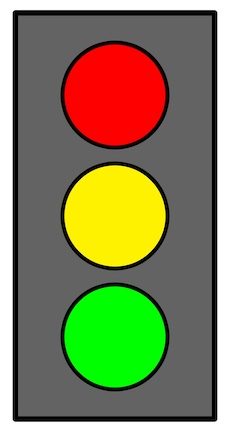
\includegraphics[scale=0.25]{ampel}
%https://www.publicdomainpictures.net/pictures/260000/velka/traffic-light-1526166819zss.jpg
\caption{Ampel.}
\label{figure-ampel}
\end{minipage}
\hfill
\begin{minipage}{0.3\textwidth}
\centering
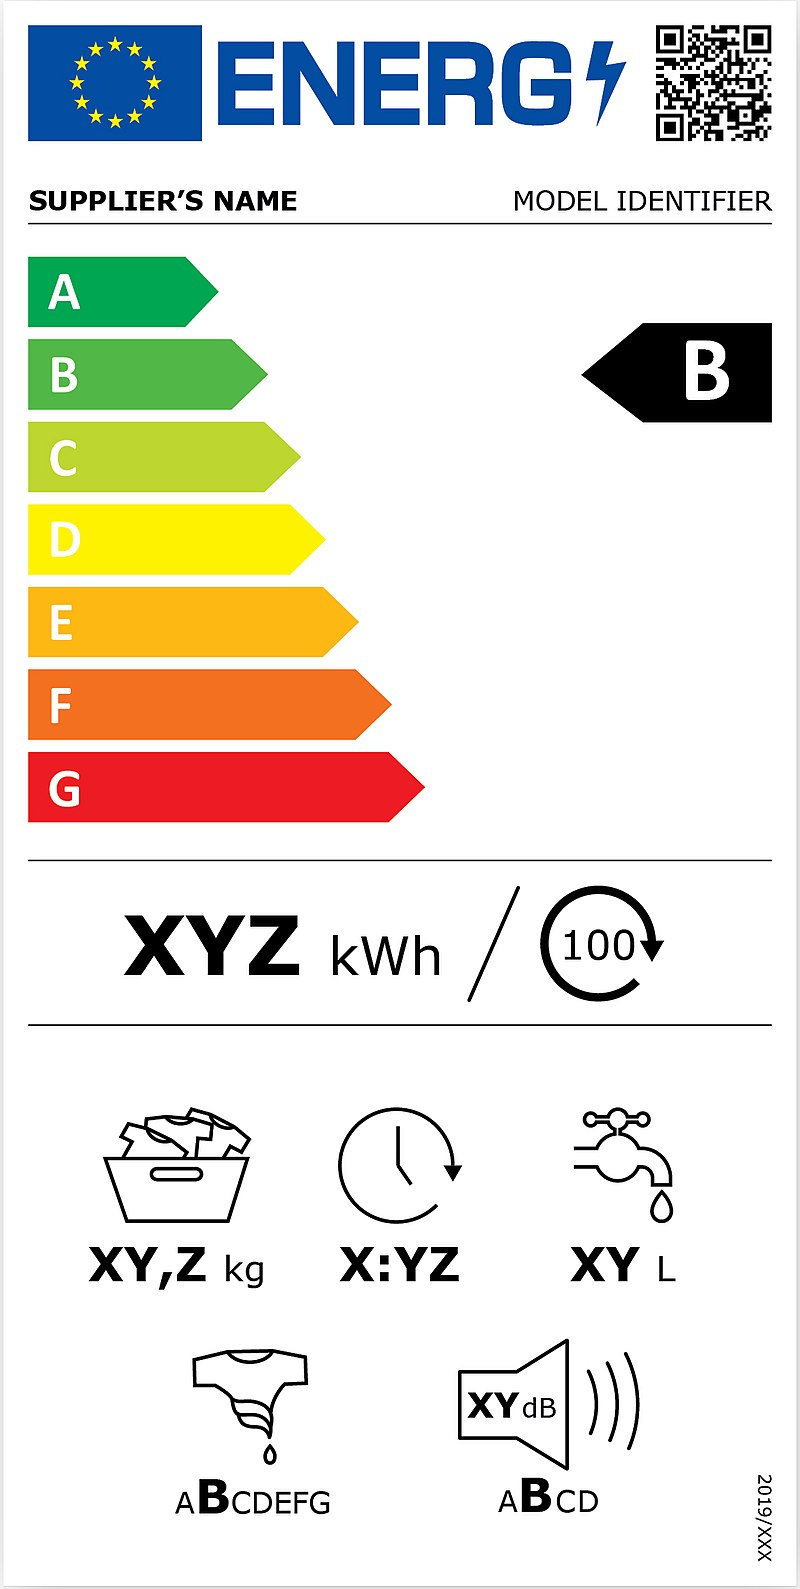
\includegraphics[scale=0.07]{eu_washing_machines_label}
%https://de.wikipedia.org/wiki/Energieverbrauchskennzeichnung#/media/Datei:EU_washing_machines_label.jpg
\caption{Energieverbrauchskennzeichnung.}
\label{figure-energie}
\end{minipage}
\hfill
\begin{minipage}{0.3\textwidth}
\centering
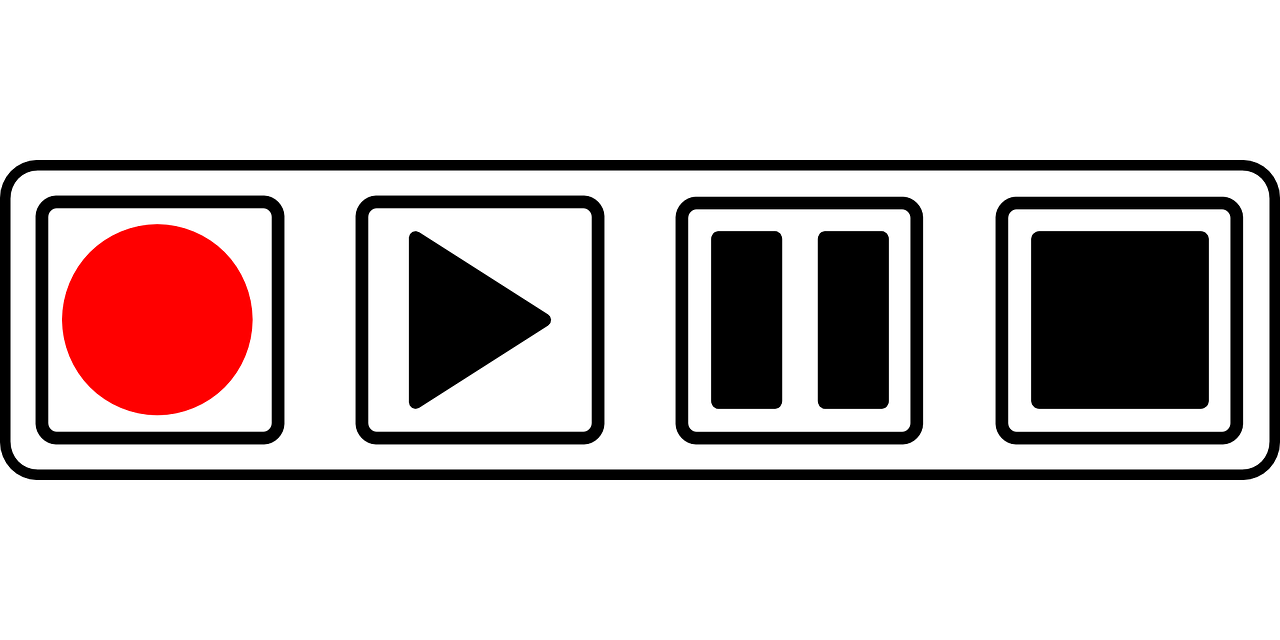
\includegraphics[scale=0.1]{start_stop_play}
%https://pixabay.com/de/vectors/tasten-anschlag-spielen-anhalten-35531/
\caption{Zeichen bei Abspielgeräten.}
\label{figure-abspielgeraet}
\end{minipage}
\end{figure}

Auch in der Informatik spielen Codierungen eine wichtige Rolle. Ohne Codierungen könnten wir nicht programmieren. Keine Bilder speichern oder Nachrichten übertragen. Wir wollen uns in diesem Kapitel mit Codierungen vertraut machen und einige wichtige Codierungen für Zahlen, Texte und Bilder anschauen, sodass der Computer diese verarbeiten kann.

\newcommand{\codierungenLernziele}{
\protect\begin{todolist}
\item Sie definieren den Begriff \say{Codierung} und \say{Decodierung}.
\item Sie erstellen einen eindeutig decodierbaren Code.
\item Sie wenden einen gegebenen Code an.
\end{todolist}
}

\lernziel{\autoref{chapter-codierungen}, \nameref{chapter-codierungen}}{\protect\codierungenLernziele}

\codierungenLernziele

\section{Definitionen und Beispiele}

Codierung bedeutet in der Informatik meistens die Umwandlung einer Information von einer Form in eine andere Form. Meist wird Information in der für den Menschen verständlichen Form in eine für Maschinen verarbeitbare Form umgewandelt. Formaler betrachtet ist das Codieren eine Zuordnung zwischen einem Alphabet und Wörtern. Dazu müssen wir zunächst die Menge aller Wörter, die man mit einem Alphabet erstellen betrachten.

\begin{definition}[Menge aller Wörter eines Alphabets]
Wir bezeichnen mit $\mathscr{A}^*$ die Menge aller Wörter über $\mathscr{A}$. $\mathscr{A}^*$ ist eine unendliche Menge. Wenn man nun $w \in \mathscr{A}^*$ schreibt, dann ist damit die Aussage \say{$w$ ist ein Wort über $\mathscr{A}$} gemeint.
\end{definition}

\begin{example}
Für $\mathscr{A}_{Bin} = \{0, 1\}$ erhalten wir: $\mathscr{A}_{Bin}^* = \{0, 1, 00, 01, 10, 11, 000, 001, 010, 011, 100,$ $101, 110, 111, 0000, \dots \}$. Für $\mathscr{A}_{a} = \{a\}$ erhalten wir: $\mathscr{A}_{a}^* = \{a, aa, aaa, aaaa, aaaaa, \dots \}$.
\end{example}

Die Beispiele verdeutlichen, dass man alle Wörter der Länge $1$, $2$, $3$, $\dots$ hintereinanderschreiben kann, wenn man Wörter über einem Alphabet auflisten möchte. Wir können die Länge der Wörter auch eingrenzen.

\begin{definition}[Menge aller Wörter gleicher Länge]
Wir bezeichnen mit $\mathscr{A}^n$ die Menge aller Wörter der Länge $n$ über $\mathscr{A}$ . $\mathscr{A}^n$ ist \textbf{keine} unendliche Menge. Wenn man nun $w \in \mathscr{A}^n$ schreibt, dann ist damit die Aussage \say{$w$ ist ein Wort der Länge $n$ über $\mathscr{A}$} gemeint.
\end{definition}

\begin{example}
Alle Binärwörter der Länge $3$: $\mathscr{A}_{Bin}^3 = \{000, 001, 010, 011, 100, 101, 110, 111\}$.
\end{example}

\subsection{Aufgaben 1}

\begin{enumerate}
\item Listen Sie die $39$ kürzesten Wörter über dem Alphabet $\mathscr{A}_{abc} = \{a, b, c\}$ auf.
\item Ist das Wort $abba$ aus $\mathscr{A}_{abc}^*$? Ist $abbdca$ aus $\mathscr{A}_{abc}^*$?
\item Es sei $w = \text{Ben}$. Gilt $w \in \mathscr{A}_{Lat}^*$?
\item Bestimmen Sie $\mathscr{A}_{a}^5$ für $\mathscr{A}_{a} = \{a\}$.
\item Ist $abbaab$ und $abbdca$ aus $\mathscr{A}_{abc}^6$?
\item Listen Sie die alle Wörter aus $\mathscr{A}_{abc}^2 = \{a, b, c\}^2$ auf.
\end{enumerate}

\begin{definition}[Codierung]
Man spricht von einer Codierung (eng. encoding), wenn jedem \textbf{Zeichen} eines Alphabets $\mathscr{A}_1$ ein \textbf{Wort} $w$ aus einem Alphabet $\mathscr{A}_2$ zugeordnet wird. Wir schreiben dafür $\mathscr{A}_1 \rightarrow \mathscr{A}_2^*$.
\end{definition}

Es geht bei der Codierung also darum, dass man Zeichen durch andere Wörter ersetzt. Wichtig bei einer Codierung ist auch die Umkehrung. Ein Codierung muss auch \textbf{eindeutig} wieder rückgängig gemacht werden können. Diesen Vorgang nennen wir \textbf{Decodierung} (eng. decoding). Wie man ein Zeichen codiert bzw. decodiert wird typischerweise durch eine Code-Tabelle festgehalten. 

\begin{example}[Morsecode]
\autoref{table-morse} zeigt einen Teil des \textbf{Morsecodes}. Wir verwenden $\mathscr{A}_{Lat} = \{A, B, C, \dots , X, Y, Z\}$. Durch die Code-Tabelle wird jedem Zeichen aus $\mathscr{A}_{Lat}$ ein Wort aus $\mathscr{A}_{Morse}^*= \{\cdot, -\}^*$ zugeordnet. Kurz notiert durch $\mathscr{A}_{Lat} \rightarrow \mathscr{A}_{Morse}^*$. 

\begin{table}[htb]
\centering
\begin{tabular}{|c|c||c|c||c|c|}
\hline
\textbf{Zeichen} & \textbf{Code-Wort} & \textbf{Zeichen} & \textbf{Code-Wort} & \textbf{Zeichen} & \textbf{Code-Wort} \\ \hline
A & $\cdot~-$ & J & $\cdot~-~-~-~$ & S & $\cdot~\cdot~\cdot$ \\ \hline
B & $-~\cdot~\cdot~\cdot$ & K & $-~\cdot~-$ & T & $-$ \\ \hline
C & $-~\cdot~-~\cdot$ & L & $\cdot~-\cdot~\cdot$ & U & $\cdot~\cdot~-$ \\ \hline
D &  $-~\cdot~\cdot$  & M & $-~-$ & V & $\cdot~\cdot~\cdot~-$ \\ \hline
E & $\cdot$ & N & $-~\cdot$ & W & $\cdot~-~-$ \\ \hline
F & $\cdot~\cdot~-~\cdot$ & O & $-~-~-~$ & X & $-~\cdot~\cdot~-$ \\ \hline
G & $-~-~\cdot$ & P & $\cdot~-~-~\cdot$  & Y & $-~\cdot~-~-$ \\ \hline
H & $\cdot~\cdot~\cdot~\cdot$ & Q & $-~-~\cdot~-$ & Z & $-~-~\cdot~\cdot~$ \\ \hline
I & $\cdot~\cdot$ & R & $\cdot~-~\cdot$ &   &  \\ \hline
\end{tabular}
\caption{Code-Tabelle für den Morsecode.}
\label{table-morse}
\end{table}

Wenn wir das Zeichen G codieren, dann erhalten wir $-~-~\cdot$. Decodieren wir das Code-Wort $-~\cdot~\cdot~-$, dann erhalten wir das Zeichen X.

\end{example}

\autoref{table-morse} sind drei Spalten mit dem Begriff \say{Code-Wort} beschriftet. Wir können diesen Begriff wie folgt festhalten:

\begin{definition}[Code-Wort und Code]
Das Wort, welches durch das Codieren entsteht, bezeichnen wir als \textbf{Code-Wort}. Die Menge aller Code-Wörter bezeichnen wir als \textbf{Code}. Bekannte Code-Wörter erhalten meist einen eigenen Codenamen.
\end{definition}

Somit bilden alle Code-Wörter aus \autoref{table-morse} einen Code - den Morsecode.

\begin{important}
Die Codierung von \textbf{einzelnen Zeichen} kann für die \textbf{Codierung von Wörtern} verwendet werden.
\end{important}

\begin{example}
Beim Morsecode werden Wörter Zeichen für Zeichen codiert. Zwischen zwei Zeichen benötigt es jedoch ein \say{Trennelement} - die Pause ($/$). Für das Wort SOS erhalten wir somit $\cdot~\cdot~\cdot~/~-~-~-~/~\cdot~\cdot~\cdot$.
\end{example}

\begin{important}
Für alle Codes gilt, dass beim Codieren kein Datenverlust auftreten darf. Wir stellen die Daten lediglich durch andere Zeichen dar.
\end{important}

\subsection{Aufgaben 2}

\begin{enumerate}
\item Decodieren das $w = \cdot~\cdot~/-~\cdot~/~\cdot~\cdot~-~\cdot~/~-~-~-~/~\cdot~-~\cdot~/~-~-~/~\cdot~-~/~-~/~\cdot~\cdot~/~-~\cdot~-$ aus $\mathscr{A}_{MorseWort}^*=\{\cdot, -\, /\}^*$.
\item Codieren Sie Ihren Vornamen mit dem Morsecode. Verwenden Sie nur Grossbuchstaben.
\end{enumerate}

\section{Binärcodes}

Ein Computer kennt zwei Zustände: Spannung oder keine Spannung. Aus diesem Grund sind wir vor allem an Codes interessiert, welche ein Alphabet mit zwei Zeichen verwenden.

\begin{definition}[Binärcode]
Falls ein Code nur Code-Wörter mit zwei Zeichen verwendet, dann handelt es sich um einen Binärcode. Üblicherweise werden die beiden Zeichen durch 0 und 1 repräsentiert.
\end{definition}

Binärcodes sind im Computerbereich deshalb üblich, da sie sich direkt durch eine Elektronik (Digitaltechnik) verarbeiten lassen, die zwei Zustände (\say{Eingeschaltet} und \say{Ausgeschaltet}) versteht. Wir fokussieren uns deshalb von nun an auf Binärcodes.

\section{Eindeutig decodierbare Codes}

Betrachten wir das Wort $0001$. Es wurde mit dem Code aus \autoref{table-geo} codiert. Welches Wort wurde für die Codierung benutzt? 

\begin{table}[htb]
\centering
\begin{minipage}{0.6\textwidth}
\centering
\begin{tabular}{|c|c|}
\hline
Zeichen & Code-Wort \\ \hline
 $\Circle$       & 0         \\ \hline
 $\Square$       & 00        \\ \hline
 $\Diamond$       & 1         \\ \hline
 $\triangle$       & 01        \\ \hline
\end{tabular}
\caption{Code-Tabelle für eine Codierung von $\mathscr{A}_{Geo}$.}
\label{table-geo}
\end{minipage}
\hfill
\begin{minipage}{0.3\textwidth}
\centering
\begin{itemize}
\item $\Circle\Circle\Circle\Diamond$
\item $\Circle\Square\Diamond$
\item $\Square\Circle\Diamond$
\item $\Square\triangle$
\item $\dots$
\end{itemize}
\end{minipage}
\end{table}

Wir wissen nicht, welches Wort korrekt ist, da mehrere mögliche Wörter beim Decodieren entstehen können. Wir sprechen nur dann von einem \textbf{eindeutig decodierbaren Code}, wenn jedes Code-Wort exakt zu einem Wort decodiert werden kann.

\begin{definition}[Eindeutig decodierbarer Code]
Ein Code heisst eindeutig decodierbar genau dann, wenn jedes Code-Wort (das heisst jedes codierte Wort) nur auf eine einzige Art zurückübersetzt (decodiert) werden kann.
\end{definition}

Es müssen dabei nur Wörter eindeutig decodierbar sein, welche zuvor korrekt codiert wurden. Nicht jedes beliebige Wort muss somit (eindeutig) decodierbar sein. Wie können wir einen eindeutig decodierbaren Code erzeugen? Eine sehr einfache Möglichkeit sind Codes bei denen \textbf{alle} Code-Wörter dieselbe Länge besitzen.

\begin{definition}[Blockcode]
Wenn wir alle Zeichen mit einer festen Länge $n$ codieren (eng. fixed length encoding), dann erhalten wir einen \textbf{Blockcode}. Jedes Code-Wort $w$ besitzt deshalb die Länge $w = n$. Wenn man jedes Code-Wort nur einmal verwendet, dann ist der Code automatisch eindeutig decodierbar. Wir schreiben für einen Blockcode, welcher die Zeichen aus dem Alphabet $\mathscr{A}_1$ codiert, $\mathscr{A}_1 \rightarrow \mathscr{A}_2^n$. Mit $\mathscr{A}_2^n$ ist gemeint, dass nur Code-Wörter der Länge $n$ verwendet werden.
\end{definition}

Ein Blockcode benötigt kein \say{Trennelement} zwischen Code-Wörtern. Durch die fixe Anzahl an Zeichen pro Code-Wörter lassen sich Code-Wörter automatisch trennen.

\section{Wie man einen binären Blockcode erstellt}

Bevor wir uns existierende Codes anschauen, geht es darum zu verstehen wie man einen binären Blockcode (wir codieren Zeichen für Zeichen) für ein Alphabet erstellen kann. Dies kann man sehr automatisiert nach folgenden Regeln erledigen:

\begin{enumerate}
\item Wie viele Zeichen des Alphabets $\mathscr{A}$ sollen codiert werden? Bestimme die Grösse von $\mathscr{A}$, das heisst $|\mathscr{A}|$.
\item Berechne die Anzahl der Bits pro Code-Wort: $log_2(|\mathscr{A}|)$ (falls es keine ganze Zahl ist, dann muss man zur \textbf{nächsten} ganzen Zahl \textbf{aufrunden}).
\item Erstelle eine Tabelle mit $|\mathscr{A}|$ Zeilen und 2 Spalten.
\item Notiere in der \textbf{ersten} Spalte alle Zeichen aus $\mathscr{A}$ (pro Zeile ein Zeichen).
\item Notiere in der \textbf{zweiten} Spalte alle Code-Wörter (pro Zeile ein Code-Wort). Wir erhalten die Code-Wörter durch \say{binäres} Zählen von $0$ bis $|\mathscr{A}|$-1. Alle Code-Wörter haben die Länge $|\mathscr{A}|$. Fülle Code-Wörter mit einer kleineren Länge mit $0$'en auf.
\end{enumerate}

Wir verbessern nun den Code aus \autoref{table-geo}. Wir erzeugen einen Blockcode.

\begin{table}[htb]
\centering
\begin{minipage}{0.6\textwidth}
\begin{example}
Wir möchten jedes Zeichen aus $\mathscr{A}_{Geo}$ codieren. Es gibt vier Zeichen ($\Circle$, $\Square$, $\Diamond$, $\triangle$) in $\mathscr{A}_{Geo}$, das heisst $|\mathscr{A}_{Geo}| = 4$. Wir benötigen also  $log_2(|\mathscr{A}_{Geo}|)=log_2(4)=2$ Bits pro Code-Wort. Wir müssen also für jedes der vier Zeichen ein Code-Wort aus zwei Bits erzeugen. Kein Code-Wort darf dabei mehrfach verwendet werden. Wir erhalten \autoref{table-geo-blockcode}.
\end{example}
\end{minipage}
\hfill
\begin{minipage}{0.35\textwidth}
\centering
\begin{tabular}{|c|c|}
\hline
Zeichen & Code-Wort \\ \hline
 $\Circle$       & 10         \\ \hline
 $\Square$       & 00        \\ \hline
 $\Diamond$       & 11         \\ \hline
 $\triangle$       & 01        \\ \hline
\end{tabular}
\caption{Code-Tabelle für den Blockcode von $\mathscr{A}_{Geo}$.}
\label{table-geo-blockcode}	
\end{minipage}
\end{table}

\begin{important}
Mit einem Blockcode $\mathscr{A}^n_{Bin}$ (ein Binärcode bei dem alle Code-Wörter $n$ Bits besitzen) lassen sich maximal $2^n$ Zeichen aus $\mathscr{A}$ codieren. Umgekehrt gilt: Möchte man $|\mathscr{A}|$ Zeichen codieren, dann benötigt man mindestens $log_2(|\mathscr{A}|)$ Bits pro Code-Wort, also einen Blockcode mit einer Mindestlänge von $log_2(|\mathscr{A}|)$ Bits.
\end{important}

\subsection{Aufgaben 3}

Wir betrachten den Morsecode aus \autoref{table-morse}.

\begin{enumerate}
\item Ist der Morsecode auch ein Blockcode? Begründen Sie Ihre Antwort.
\item Beim Morsecode können keine zwei Code-Wörter verwechselt werden. Jedes Code-Wort ist somit eindeutig decodierbar. Wodurch gelingt dies?
\item Wie wird beim Morsecode sichergestellt, dass eine Folge von Code-Wörtern eindeutig decodierbar sind?
\item Erstellen Sie einen binären Blockcode für $\mathscr{A}_{Arrows} = \{$\faAngleDoubleDown, \faAngleDoubleLeft, \faAngleDoubleRight, \faAngleDoubleUp, \faAngleDown, \faAngleLeft, \faAngleRight, \faAngleUp $\}$.
\end{enumerate}

\section{Numerische Codes}

In diesem Abschnitt betrachten wir drei Möglichkeiten wie man dezimale Zahlen durch Binärziffern darstellen kann. Wir untersuchen somit die Zuordnung $\mathscr{A}_{Dez} \rightarrow \mathscr{A}_{Bin}^*$ beziehungsweise $\mathscr{A}_{Dez}^* \rightarrow \mathscr{A}_{Bin}^*$.

\subsection{Dualcode}

Dieser Code entspricht der Umwandlung einer natürlichen Zahl aus dem Zehnersystem (Dezimalsystem) in das Zweiersystem (Dualsystem). Diesen Code kann man nicht in einer Code-Tabelle angeben, da es unendlich viele natürliche Zahlen gibt. Die Codierung erfolgt mit einer Rechnung. Sowohl die Zahlen aus dem Dezimalsystem, als auch die Zahlen aus dem Dualsystem arbeiten mit Stellenwert.
Bei dieser Codierung wird jedem Wort aus $\mathscr{A}_{Dez}^*$ ein Wort aus $\mathscr{A}_{Bin}^*$ zugeordnet. \autoref{table-dezimalzahlen-dualzahlen} zeigt ein paar Beispiele. \autoref{chapter-dualsystem} beschreibt das Codierungsverfahren im Detail.

\begin{table}[htb]
\centering
\begin{tabular}{|l|l|l|l|}
\hline
Dezimalzahl & Dualzahl & Dezimalzahl & Dualzahl    \\ \hline
0           & 0        & 21          & 10101       \\ \hline
1           & 1        & 42          & 101010      \\ \hline
12          & 1100     & 1024        & 10000000000 \\ \hline
\end{tabular}
\caption{Ausgewählte Dezimalzahlen und Dualzahl.}
\label{table-dezimalzahlen-dualzahlen}
\end{table}

Bei dieser Codierung handelt es sich typischerweise \textbf{nicht} um einen Blockcode. Mehrere Zahlen müssen durch ein  Trennelement unterschieden werden.

\subsection{BCD-Code}

Jeder Dezimalziffer wird beim \acf{BCD}-Code ein Wort aus $\mathscr{A}_{Bin}^4$ zugeordnet. Wir haben somit einen Code, der jedes Zeichen aus $\mathscr{A}_{Dez}$ codiert ($\mathscr{A}_{Dez} \rightarrow \mathscr{A}_{BCD} = \mathscr{A}_{Bin}^4$). Jede Dezimalziffer wird isoliert mittels Dualcode übersetzt (siehe \autoref{table-bcd}).

\begin{table}[htb]
\centering
\begin{tabular}{|c|c|c|c|c|c|c|c|}
\hline
Zeichen & Code-Wort & Zeichen & Code-Wort & Zeichen & Code-Wort & Zeichen & Code-Wort \\ \hline
0       &   0000        & 5       &   0101        &         &  1010   &         &  1111      \\ \hline
1       &   0001        & 6       &   0110        &         &  1011   & &     \\ \hline
2       &   0010        & 7       &   0111        &         &  1100    & &     \\ \hline
3       &   0011        & 8       &   1000        &         &  1101    & &    \\ \hline
4       &   0100        & 9       &   1001        &         &  1110    & &     \\ \hline
\end{tabular}
\caption{Code-Tabelle für den \ac{BCD}-Code.}
\label{table-bcd}
\end{table}

Da es zehn Dezimalziffern gibt, benötigen wir Code-Wörter der Länge vier. Das heisst, jedes Code-Wort besteht aus vier Bits. Es ist also ein Blockcode.

\begin{hinweis}
Möchte man zehn Zeichen eindeutig mit einem Alphabet von zwei Zeichen codieren, dann benötigt man pro Code-Wort mindestens $log_2(10) \approx 3,32$ Bits. Da es nur \say{ganze} Bits gibt, müssen wir $3,32$ aufrunden und erhalten 4 Bits pro Code-Wort.
\end{hinweis}

Bei diesem Code gibt es mehr Code-Wörter als Zeichen. Einige Code-Wörter (z.B. $1101$) werden nicht \say{gebraucht}. Diese Code-Wörter codieren kein gültiges Zeichen und dürfen nicht verwendet werden. Eine natürliche Zahl wird dann Dezimalziffer für Dezimalziffer codiert. Die Zahl $42$ wird somit zu $01000010$ codiert. Der \ac{BCD}-Code findet in der Praxis nur noch selten eine Anwendung. Bei einer \ac{SMS}-Nachricht wird die Telefonnummer mittels \ac{BCD}-Code codiert.

\subsubsection{Aufgaben 4}

\begin{enumerate}
\item Codieren Sie die Zahl $65536$ mit dem \ac{BCD}-Code. Wie viele Bits werden benötigt? Wie viele Bits benötigt man für die Zahl, wenn man den Dualcode verwenden würde?
\item Decodieren Sie das Wort $0010000000000001$ unter der Verwendung des \ac{BCD}-Codes.
\end{enumerate}

\subsection{1-aus-n Code}

Jede Dezimalziffer wird mit $n$ Bits codiert. Es ist also ein Blockcode mit Code-Wörtern der Länge $n$ ($\mathscr{A}_{Dez} \rightarrow \mathscr{A}_{Bin}^n$). Beim Codieren wird für jede Dezimalziffer pro Code-Wort nur eine $1$ verwendet. Alle anderen Bits sind $0$. Typischerweise werden $10$ Bits verwendet, da man $10$ Dezimalziffern hat. Es ergibt sich somit ein 1-aus-10 Code ($\mathscr{A}_{Dez} \rightarrow \mathscr{A}_{\text{1-aus-10}} = \mathscr{A}_{Bin}^{10}$). Man beginnt bei der Dezimalziffer $0$ und setzt dafür das Bit ganz \say{rechts} im Code-Wort auf $1$ (\say{das $0$. Bit}). Alle anderen Bits werden auf 0 gesetzt. Für die anderen Dezimalziffern fährt man analog fort. Die Dezimalziffer $1$ erhält somit im Code-Wort beim $1$. Bit eine $1$. Die Dezimalziffer $2$ erhält somit im Code-Wort beim $2$. Bit eine $1$ usw. Wir fassen den 1-aus-10 Code als Code-Tabelle zusammen (siehe \autoref{table-1-aus-10}).

\begin{table}[htb]
\centering
\begin{tabular}{|c|c|c|c|}
\hline
Zeichen & Code-Wort & Zeichen & Code-Wort \\ \hline
0       &   0000000001        & 5       &   0000100000        \\ \hline
1       &   0000000010        & 6       &   0001000000        \\ \hline
2       &   0000000100        & 7       &   0010000000        \\ \hline
3       &   0000001000        & 8       &   0100000000        \\ \hline
4       &   0000010000        & 9       &   1000000000        \\ \hline
\end{tabular}
\caption{Code-Tabelle für den 1-aus-10 Code.}
\label{table-1-aus-10}
\end{table}

Der 1-aus-10 Code benutzt nur einen Bruchteil der möglichen Code-Wörter. Alle anderen Code-Wörter sind nicht erlaubt. Eine natürliche Zahl wird dann Dezimalziffer für Dezimalziffer codiert. Die Zahl $42$ wird somit zu $00000100000000000100$ codiert. Der 1-aus-n-Code findet in der Praxis bei Speicherchips seine Anwendung.

\subsubsection{Aufgaben 5}

\begin{enumerate}
\item Codieren Sie die Zahl $65536$ mit dem 1-aus-10-Code. Wie viele Bits werden benötigt? Wie viele Bits benötigt man für die Zahl, wenn man den Dualcode verwenden würde?
\item Decodieren Sie das Wort $0000000100000000000100000000010000000010$ unter der Verwendung des 1-aus-10 Codes.
\item Wie viele Code-Wörter sind beim 1-aus-10 Code nicht erlaubt?
\end{enumerate}

\newpage

\section{Alphanumerische Codes}
\label{section-alphanumerische-codes}

Wir möchten in diesem Abschnitt nun ein alphanumerisches Zeichen codieren. Ein alphanumerisches Zeichen entspricht im weiteren Sinn einem Zeichen aus $\mathscr{A}_{Tastatur}$. Wir möchten zum Beispiel das Zeichen \texttt{A}, \texttt{@} oder \texttt{7} (als Zeichen, nicht als Ziffer!), welche man auf einer üblichen Tastatur findet, codieren. Ziel der Codierungen ist es, dass wir einen Text in einer Textdatei auf dem Computer abspeichern können. Wir müssen also Code-Wörter aus $\mathscr{A}_{Bin}^*$ erzeugen. 

Die Lernziele für diesen Abschnitt lauten (zu den bereits erwähnten Lernzielen) wie folgt:

\newcommand{\alphabnumerischeCodesLernziele}{
\protect\begin{todolist}
\item Sie erklären, warum es für gewisse Codierungen einen Standard gibt.
\item Sie nennen und erklären bekannte Codes.
\end{todolist}
}

\lernziel{\autoref{section-alphanumerische-codes}, \nameref{section-alphanumerische-codes}}{\protect\alphabnumerischeCodesLernziele}

\alphabnumerischeCodesLernziele

Grundlegend gilt für alle Codes, dass beim Datenaustausch (siehe \autoref{figure-datenaustausch}) zwischen zwei Maschinen (z.B. eine Textdatei wird zwischen zwei Computern ausgetauscht), beiden Maschinen das benutzte Datenformat bekannt sein muss. Sonst kann der Empfänger die Daten nicht erfolgreich lesen. Wenn man eine Textdatei erstellt, dann benutzt das Programm einen bekannten Code.

\begin{figure}[htb]
\centering
\begin{minipage}{0.15\textwidth}
\centering

\includegraphics[scale=0.1]{notebook}
\end{minipage}
$\overbrace{\Longleftrightarrow}^{\texttt{010011010010}}$
\begin{minipage}{0.15\textwidth}
\centering

\includegraphics[scale=0.1]{notebook}
\end{minipage}
\caption{Zwei Computer tauschen Daten aus.}
\label{figure-datenaustausch}
\end{figure}

Der Sender schickt die Textdatei an den Empfänger. Der Empfänger öffnet dann die Textdatei. Das Programm zum Öffnen der Textdatei muss den benutzten Code des Senders verstehen. Nur wenn Sender und Empfänger denselben Code für die Textdatei verwenden, ist ein erfolgreicher Datenaustausch möglich. Sonst kann der Empfänger den Inhalt der Textdatei nicht lesen. Beide müssen also einen Code vereinbaren. Damit nicht jeder seinen eigenen Code vereinbaren muss, gibt es verschiedene \textbf{Standards} für die Codierung von alphanumerischen Zeichen. Ein Standard für die Codierung steht allen Maschinen und Programmen frei zur Verfügung und soll die Kommunikation erleichtern. Wir schauen uns in den folgenden Abschnitten einige Standards an.

\begin{figure}[htb]
\centering
\caption*{\footnotesize STANDARDS (\url{https://xkcd.com/927/})}
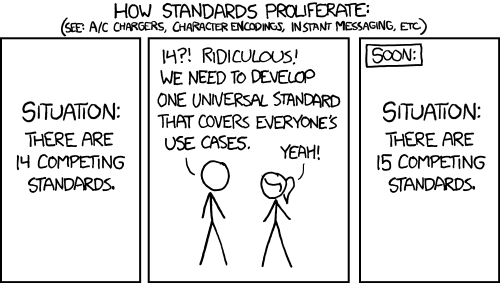
\includegraphics[scale=0.5]{standards}
\caption*{\footnotesize Fortunately, the charging one has been solved now that we've all standardized on mini-USB. Or is it micro-USB? Shit.}
\end{figure}

\begin{hinweis}
Ein Standard (auch Norm) genannt gibt es auch in anderen Gebieten. Es gibt zum Beispiel standardisierte Papierformate (z.B. \ac{DIN} A4) oder Buchnummern (geregelt durch die Internationale Organisation für Normung\footnote{Meist als ISO (von griechisch isos (dt. gleich)) bezeichnet.}. Standards befinden sich auch in einem Entwicklungsprozess. Ein Beispiel dafür ist die Entwicklung eines einheitlichen Ladekabels für Handys. Manchmal gibt es auch Standards die in Konkurrenz zueinander stehen (zum Beispiel \ac{HDMI} und DisplayPort zur Übertragung von Bild und Ton).
\end{hinweis}

Eine Codierung von alphanumerischen Zeichen wird auch \textbf{Zeichencodierung} (eng. character encoding) genannt. Mit Zeichen sind hier Schriftzeichen oder Symbole gemeint. Bevor wir uns drei Standards anschauen, zeigen wir die Idee mit einem \say{kleinen} Alphabet.

\begin{example}
Als \say{Eingangsbeispiel} möchten wir $\mathscr{A}_{Lat} = \{A, B, C, \dots, X, Y, Z\}$ codieren. Es geht also darum, wie man für jedes Zeichen aus $\mathscr{A}_{Lat}$ ein Code-Wort aus $\mathscr{A}_{Bin}^*$ erzeugen kann (binärer Blockcode: $\mathscr{A}_{Lat} \rightarrow \mathscr{A}_{Bin}^*$).

$\mathscr{A}_{Lat}$ besteht aus $26$ Zeichen, das heisst $|\mathscr{A}_{Lat}| = 26$. Jedes Code-Wort benötigt somit $5$ Bits (da $log_2(|\mathscr{A}|)=log_2(26)\approx4.7$). \autoref{table-code-lat} zeigt den vollständigen Code. Alle Code-Wörter sind $5$ Bits lang. Wir beginnen mit dem Code-Wort $00000$. Wir zählen dann \say{binär}, das heisst dualcodiert, bis $25$.

\begin{table}[htb]
\centering
\begin{tabular}{|c|c||c|c||c|c||c|c|}
\hline
\footnotesize
\textbf{Zeichen} & \footnotesize \textbf{Code-Wort} & \footnotesize \textbf{Zeichen} & \footnotesize \textbf{Code-Wort} & \footnotesize \textbf{Zeichen} & \footnotesize \textbf{Code-Wort} & \footnotesize \textbf{Zeichen} & \footnotesize \textbf{Code-Wort} \\ \hline
A & $00000$ & H & $00111$ & O & $01110$ & V & $10101$ \\ \hline
B & $00001$ & I & $01000$ & P & $01111$ & W & $10110$ \\ \hline
C & $00010$ & J & $01001$ & Q & $10000$ & X & $10111$ \\ \hline
D & $00011$ & K & $01010$ & R & $10001$ & Y & $11000$ \\ \hline
E & $00100$ & L & $01011$ & S & $10010$ & Z & $11001$ \\ \hline
F & $00101$ & M & $01100$ & T & $10011$ & & \\ \hline
G & $00110$ & N & $01101$ & U & $10100$ & & \\ \hline
\end{tabular}
\caption{Die Code-Wörter $11010$, $11011$, $11100$, $11101$, $11110$, $11111$ gehören nicht zum Code und dürfen nicht benutzt werden. Aus Platzgründen wurde die Tabelle in vier Teile aufgeteilt.}
\label{table-code-lat}
\end{table}

\end{example}

\subsubsection{Aufgaben 6}

\begin{enumerate}
\item Codieren Sie das Wort MENSA mit dem Code aus \autoref{table-code-lat}.
\item Decodieren Sie das Wort $00000000010000100000$ mit dem Code aus \autoref{table-code-lat}.
\end{enumerate}

\subsection{\acs{ASCII}}

Der Code umfasst das lateinische Alphabet (Gross- und Kleinbuchstaben), die zehn Dezimalziffern, Satzzeichen, Leerzeichen und weitere Sonderzeichen (z.B. das Dollar-Zeichen $\$$). Die Zeichen bilden im Wesentlichen die Tasten einer englischen Tastatur (US-Layout) ab. Neben diesen \say{sichtbaren} Zeichen (man sagt druckbare Zeichen, da der Drucker diese auf ein Blatt Papier drucken kann\footnote{Das Leerzeichen wird auch durch den Drucker abgedeckt, in dem er für das Zeichen nichts druckt}), gibt es auch noch \textbf{Steuerzeichen}. Steuerzeichen können nicht dargestellt werden (nicht druckbar). Früher wurden die Steuerzeichen zur Steuerung von Geräten (z.B. Drucker oder Fernschreiber) verwendet. Heute werden nur noch wenige Steuerzeichen verwendet. Die wichtigsten Steuerzeichen sind:

\begin{itemize}
\item ACK (Acknowledge): Empfangsbestätigung einer Nachricht.
\item BS (Backspace): Rücksetzen des Cursors.
\item HT (Horizontal Tab): \say{Tabulator-Taste}.
\item LF (Line Feed): Zeilenvorschub (\say{Enter}, Cursor springt in die nächste Zeile).
\item ESC (Escape): Abbruch, Trennung, Umschaltung.
\item DEL (Delete): Löschen.
\end{itemize}

Es gibt insgesamt $33$ Steuerzeichen und $95$ druckbare Zeichen. \ac{ASCII} codiert somit 128 Zeichen. Wir bezeichnen das Alphabet von \ac{ASCII} mit $\mathscr{A}_{ASCII}$. \autoref{table-ascii} zeigt alle Zeichen und die dazugehörigen Code-Wörter. \ac{ASCII} ist ein binärer Blockcode mit $7$ Bits (Rechenweg: $log_2(|\mathscr{A}_{ASCII}|)=log_2(128)=7$). Der Code wurde in den 1960er-Jahren entwickelt und wird auch heute noch eingesetzt.

\subsubsection{Aufgaben 7}

\begin{enumerate}
\item Codieren Sie Ihre KSWE E-mailadresse mit \ac{ASCII} .
\item Decodieren Sie 0110010011000001100000110001011101001000001000001010000010100\\11111000011000011100011110010101000001001111110010011110011110011111001111\\001011111001 mit \ac{ASCII}.
\item Wie funktioniert die kompakte Darstellung von \ac{ASCII} (siehe \autoref{table-ascii-compact})?
\end{enumerate}

\begin{table}[htb]
\centering
\begin{tabular}{|c|c|c|c|c|c|c|c||c|}
\hline
\multicolumn{9}{|c|}{Bitpositionen} \\ \hline
\multicolumn{8}{|c||}{7, 6, 5} & 4, 3, 2, 1 \\ \hline \hline
000 & 001 & 010 & 011 & 100 & 101 & 110 & 111 & \\\hline 
NUL & DLE & $\sqcup$  & 0   & @   & P   &  `   &  p & 0000    \\ \hline 
SOH  & DC1   &  !   &  1   &  A   &  Q   &  a   &  q & 0001     \\ \hline 
STX   &  DC2    &   "   &   2  &  B   &  R   &  b   &  r & 0010     \\ \hline 
ETX   &  DC3    &  \#   &  3   &  C   &  S   &  c   &  s & 0011     \\ \hline 
EOT   & DC4    &  \$   &  4   &  D   &  T   &  d   &  t & 0100     \\ \hline 
ENQ  & NAK    &  \%   &  5   &  E   &  U   & e    & u & 0101      \\ \hline 
ACK  & SYN    & \&    &  6   &  F   &  V   &  f   &  v & 0110    \\ \hline 
BEL   & ETB   & ‘     &   7 &  G   &  W   &  g   &  w & 0111    \\ \hline 
BS   &  CAN   &  (    &  8   & H    & X    &  h   &  x & 1000    \\ \hline 
HT   &  EM   &  )   &  9   &  I   &  Y   &  i   &  y & 1001     \\ \hline 
LF   &  SUB   &  *   & :    &  J   &  Z   & j    & z & 1010     \\ \hline 
VT   &   ESC  &  +   & ;    &  K   &  [   & k    & \{ & 1011      \\ \hline 
FF   & FS    &  ,   & <    &  L   &  \textbackslash   &  l   &  | & 1100    \\ \hline 
CR   &  GS   &  -   & =    & M    &  ]   & m    &  \}  & 1101   \\ \hline 
SO   &  RS   &  .   &  >   &  N   &  \textasciicircum   &  n   &  \textasciitilde  & 1110   \\ \hline 
SI  &  US   &   /  &  ?   &  O   &  \_   & o    & DEL & 1111    \\ \hline
\end{tabular}
\caption{Kompakte Notation von \ac{ASCII}.}
\label{table-ascii-compact}
\end{table}

\begin{table}[!htbp]
\centering
\begin{tabular}{|c|r|r||c|r|r||r|r|r|}
\hline
Zeichen & Dez & Code-Wort & Zeichen & Dez & Code-Wort & Zeichen          & Dez & Code-Wort \\ \hline
\hline
NUL     & 0       	& 0000000     & +       & 43      		& 0101011           & V                & 86      	& 1010110           \\ \hline
SOH     & 1       & 0000001         & ,       & 44     		& 0101100          & W                & 87      	& 1010111         \\ \hline
STX     & 2       	& 0000010        & -       & 45      		& 0101101          & X                & 88      	& 1011000          \\ \hline
ETX     & 3       	& 0000011        & .       & 46      		& 0101110         & Y                & 89      	& 1011001          \\ \hline 
EOT     & 4       	& 0000100          & /       & 47   		& 0101111          & Z                & 90      	& 1011010          \\ \hline
ENQ     & 5       & 0000101          & 0       & 48   		& 0110000          & [                & 91      	& 1011011          \\ \hline
ACK     & 6       & 0000110           & 1       & 49  		& 0110001          & \textbackslash   & 92  	& 1011100          \\ \hline
BEL     & 7       	& 0000111          & 2       & 50  		& 0110010          & ]                & 93      	& 1011101          \\ \hline
BS      & 8       	& 0001000         & 3       & 51   		& 0110011          & \textasciicircum & 94   	& 1011110          \\ \hline
HT     & 9       	& 0001001          & 4       & 52  		& 0110100          & \_               & 95      	& 1011111         \\ \hline
LF      & 10      	& 0001010           & 5       & 53      	& 0110101          & `                & 96      	& 1100000          \\ \hline
VT      & 11      	& 0001011          & 6       & 54      	& 0110110          & a                & 97      	& 1100001          \\ \hline
FF      & 12      	& 0001100         & 7       & 55      	& 0110111          & b                & 98      	& 1100010         \\ \hline
CR      & 13      	& 0001101           & 8       & 56      	& 0111000          & c                & 99      	& 1100011          \\ \hline
SO      & 14      	& 0001110          & 9       & 57      	& 0111001          & d                & 100     	& 1100100          \\ \hline
SI      & 15      	& 0001111          & :       & 58      	& 0111010          & e                & 101     	& 1100101          \\ \hline
DLE     & 16      & 0010000         & ;       & 59      	& 0111011          & f                & 102     	& 1100110          \\ \hline
DC1     & 17      & 0010001          & <       & 60      	& 0111100          & g                & 103     	& 1100111          \\ \hline
DC2     & 18      & 0010010          & =       & 61      	& 0111101          & h                & 104     	& 1101000         \\ \hline
DC3     & 19      & 0010011          & >       & 62      	& 0111110          & i                & 105     	& 1101001          \\ \hline
DC4     & 20      & 0010100         & ?       & 63      	& 0111111          & j                & 106     	& 1101010          \\ \hline
NAK     & 21     	& 0010101          & @       & 64      	& 1000000          & k                & 107     	& 1101011         \\ \hline
SYN     & 22     	& 0010110         & A       & 65      	& 1000001          & l                & 108     	& 1101100         \\ \hline
ETB     & 23      & 0010111          & B       & 66      	& 1000010          & m                & 109    	& 1101101         \\ \hline
CAN     & 24     & 0011000         & C       & 67      	& 1000011          & n                & 110     	& 1101110          \\ \hline
EM      & 25      	& 0011001         & D       & 68      	& 1000100          & o                & 111     	& 1101111          \\ \hline
SUB     & 26     	& 0011010         & E       & 69      	& 1000101          & p                & 112     	& 1110000          \\ \hline
ESC     & 27    	& 0011011         & F       & 70      	& 1000110          & q                & 113     	& 1110001          \\ \hline
FS      & 28      	& 0011100          & G       & 71      	& 1000111          & r                & 114     	& 1110010          \\ \hline
GS      & 29      	& 0011101          & H       & 72      	& 1001000          & s                & 115     	& 1110011         \\ \hline
RS      & 30     	& 0011110          & I       & 73      	& 1001001          & t                & 116     	& 1110100          \\ \hline
US      & 31      	& 0011111          & J       & 74      	& 1001010          & u                & 117     	& 1110101          \\ \hline
$\sqcup$ & 32 	& 0100000          & K       & 75      	& 1001011          & v                & 118     	& 1110110          \\ \hline
!       & 33      	& 0100001         & L       & 76      	& 1001100          & w                & 119     	& 1110111          \\ \hline
"       & 34      	& 0100010          & M       & 77      	& 1001101          & x                & 120     	& 1111000         \\ \hline
\#      & 35      	& 0100011          & N       & 78      	& 1001110          & y                & 121     	& 1111001          \\ \hline
\$      & 36      	& 0100100          & O       & 79      	& 1001111          & z                & 122     	& 1111010         \\ \hline
\%      & 37      	& 0100101          & P       & 80      	& 1010000          & \{               & 123     	& 1111011          \\ \hline
\&      & 38      	& 0100110          & Q       & 81      	& 1010001          & |                & 124     	& 1111100          \\ \hline
‘     & 39      	& 0100111          & R       & 82      	& 1010010          & \}               & 125     	& 1111101          \\ \hline
(       & 40      	& 0101000          & S       & 83      	& 1010011         & \textasciitilde  & 126  	& 1111110          \\ \hline
)       & 41      	& 0101001          & T       & 84      	& 1010100          & DEL                & 127     	& 1111111          \\ \hline
*       & 42      	& 0101010          & U       & 85      	& 1010101          &                  &         	&           \\ \hline
\end{tabular}
\caption{Die Dezimal-Spalte (Dez) wurde hinzugefügt, da dies die Gespräche über die \ac{ASCII}-Tabelle einfacher macht.}
\label{table-ascii}
\end{table}

\clearpage

\subsection{Latin-1}
Da mit \ac{ASCII} nicht alle Schriftzeichen der Menschen dargestellt werden können, gibt es noch weitere Codes. Bereits für die deutsche Sprache fehlen bei \ac{ASCII} die Code-Wörter für die Umlaute (ä, ö und ü). Deshalb wurde ISO 8859 erstellt. Dies ist eine Sammlung (man sagt auch Familie) von $8$-Bit-Codes. Der Standard ISO 8859-1 Code ist besser bekannt als \textbf{Latin-1} und stellt eine Erweiterung von \ac{ASCII} dar. Der Code wird hinsichtlich einiger westeuropäischer Zeichen erweitert (z.B. à, å oder ü). Jedes Code-Wort besitzt $8$ Bits. Die \ac{ASCII} Code-Wörter von $0100000$ ($=32$, $\sqcup$) bis $1111110$ ($126$, \textasciitilde) wurden übernommen und mit einer führenden Null ergänzt. Aus $1111110$ wird somit $01111110$. Ab $10100000$ ($=160$) folgen dann bis $11111111$ ($=255$) die neuen Zeichen von Latin-1.

\begin{table}[htb]
\centering
\begin{tabular}{|c|c|c|c|c|c||c|}
\hline
\multicolumn{7}{|c|}{Bitpositionen} \\ \hline
\multicolumn{6}{|c||}{8, 7, 6, 5} & 4, 3, 2, 1 \\ \hline \hline
1010 & 1011 & 1100 & 1101 & 1110 & 1111 & \\\hline
NBSP & ° & À & Ð & à & ð & 0000 \\ \hline 
¡   &  ±  &  Á   &  Ñ   &  á   &   ñ & 0001  \\ \hline 
¢   &  ²   &  Â   &   Ò  &   â  &   ò   & 0010   \\ \hline 
£   &  ³   &  Ã   &   Ó  &  ã   &    ó   & 0011    \\ \hline 
¤   &  ´   &  Ä   &   Ô  &  ä  &    ô  & 0100     \\ \hline 
¥   & µ    &  Å   &  Õ  &  å   &   õ    & 0101    \\ \hline 
¦   &   ¶  &  Æ   &  Ö  &  æ  &    ö   & 0110     \\ \hline 
§   &  ·   &  Ç   &  ×   &   ç  &   ÷   & 0111     \\ \hline 
¨   &  ¸   &   È  &   Ø  & è    &   ø    & 1000    \\ \hline 
©   &  ¹   &  É   &  Ù  &  é  &  ù   & 1001   \\ \hline 
ª   & º   & Ê   &  Ú  & ê   &  ú   & 1010       \\ \hline 
«   &  »   & Ë    &  Û   &  ë   &  û   & 1011      \\ \hline 
¬   &  ¼   & Ì    & Ü   & ì    &   ü   & 1100     \\ \hline 
SHY &  ½   &  Í   &  Ý   &  í   & ý   & 1101   \\ \hline 
®   &   ¾  &  Î   & Þ    &   î  &    þ   & 1110    \\ \hline 
¯   &  ¿   &  Ï   &  ß  &  ï   &   ÿ   & 1111     \\ \hline
\end{tabular}
\caption{Kompakte Notation von Latin-1.}
\label{table-latin-1-compact}
\end{table}

Die Steuerzeichen aus \ac{ASCII} sind im Latin-1 Code nicht vorhanden. Ausserdem gibt es einen Bereich von $33$ Code-Wörtern ($10001111$ bis $10011111$) die ebenfalls nicht benutzt werden. Latin-1 wird immer seltener benutzt. \autoref{table-latin-1-usage} zeigt den Anteil der Websites die Latin-1 zur Codierung benutzen.

\begin{table}[htb]
\centering
\small
\begin{tabular}{|c|c|c|c|c|c|c|c|c|c|c|c|}
\hline
2010   & 2011   & 2012   & 2013   & 2014   & 2015  & 2016  & 2017  & 2018  & 2019  & 2020  & 2021 \\ \hline
28.6\% & 22.0\% & 17.2\% & 13.5\% & 10.8\% & 9.3\% & 6.9\% & 5.5\% & 4.3\% & 3.6\% & 1.6\% & 1.4\%       \\ \hline
\end{tabular}
\normalsize
%https://w3techs.com/technologies/history_overview/character_encoding/ms/y
\caption{Anteil der Websites die ISO-8859-1 (Latin-1) als Codierung verwenden.}
\label{table-latin-1-usage}
\end{table}

Als De-Facto-Standard für Websites hat sich der Code aus dem nächsten Abschnitt durchgesetzt.

\subsection{Unicode}

Dieser Codierungsstandard hat das Ziel die Schriftzeichen aller Kulturen zu berücksichtigen und unter einem Dach zu vereinen. Der Code wird kontinuierlich erweitert und neue Versionen erscheinen regelmässig. Im März 2020 ist die Version 13.0 von Unicode erschienen. Es kamen $5930$ neue Zeichen hinzu (darunter sind $55$ neue Emojis) und der Code umfasst nun $143.859$ Zeichen. Unicode ist so konzipiert, dass auch in der Zukunft noch mehr Zeichen aufgenommen werden können. Der Code hat \say{Platz} für insgesamt $1.114.112$ Code-Wörter. Somit sind zurzeit knapp $13~\%$ aller Code-Wörter benutzt. Der Standard bezeichnet Code-Wörter als Code Points (dt. Codepunkte). \autoref{table-unicode} zeigt fünf Zeichen aus dem Unicode und die dazugehörigen Code Points (Code-Wörter). Die Unicode Arbeitsgemeinschaft kümmert sich auch um die Aufnahme neuer Emojis. Man kann einen Vorschlag für ein neues Emoji einreichen. Die Arbeitsgemeinschaft prüft dann die Aufnahme in den Standard.

\begin{table}[htb]
\begin{tabular}{|c|r|r|r|c|}
\hline
Zeichen & Code Point & Binär                & Dezimal & Beschreibung               \\ \hline
ß       & U+00DF     & 0000000011011111     & 223     & \footnotesize LATIN SMALL LETTER SHARP S \\ \hline
€       & U+20AC     & 0010000010101100     & 8364    & \footnotesize EURO SIGN                  \\ \hline
©       & U+00A9     & 0000000010101001     & 169     & \footnotesize COPYRIGHT SIGN             \\ \hline
\rule{0pt}{15pt} 
\includegraphics[scale=0.1]{emoji_grinning_face} & U+1F600    & 00011111011000000000 & 128512  & \footnotesize GRINNING FACE              \\ \hline
A & U+0041    & 0000000001000001 & 65  & \footnotesize LATIN CAPITAL LETTER A             \\ \hline
\end{tabular}
\caption{Die Hexadezimaldarstellung von Code Points wird durch Voranstellen von $U+$ gekennzeichnet. Mit U+00DF ist somit 00DF$_{16}$ gemeint.}
\label{table-unicode}
\end{table}

Unicode erweitert \ac{ASCII} und ist in der Lage ein Code-Wort aus \ac{ASCII} zu \say{verstehen}. Ein \ac{ASCII} Code-Wort besteht aus $7$ Bits. Das Zeichen A hat zum Beispiel das Code-Wort $1000001$. Unicode verwendet für das A den Code Point U+0041. Die letzten Bits von $0000000010101001$ ($=$ U+0041) stimmen somit mit \ac{ASCII} überein.\\
Code Points werden nicht alle mit der gleichen Länge notiert. Alle Code Points werden mindestens mit vier Hexadezimalziffern notiert. Führende Ziffern gegebenenfalls mit $0$ aufgefüllt. Korrekt wäre eigentlich, wenn man alle Code Points mit einer einheitlichen Länge von sechs Hexadezimalziffern notiert. Der \say{kleinste} Code Point wäre somit U+000000 und der \say{grösste} Code Point U+10FFFF.

\begin{figure}[htb]
\centering
\caption*{THE HISTORY OF UNICODE (\url{https://xkcd.com/1953/})}

\includegraphics[scale=0.325]{the_history_of_unicode_2x}
\caption*{2048: "Great news for Maine—we're once again an independent state!!! Thanks, @unicode, for ruling in our favor and sending troops to end New Hampshire's annexation.\protect
\includegraphics[scale=0.25]{xkcd_title_emojis}"}
\end{figure}